%2720
\newpage
\subsection{例題4-13 \ruby{照度}{しょう|ど}センサーの値をもとに絵を動かそう}

\begin{description}
    \item \textgt{\bf 考え方}
\end{description}

センサーボードのボタンだけでなく、\ruby{照度}{しょう|ど}センサーを使うこともできます。

照度センサーがどのような機能を持っているか、確認しておきましょう。


ファイル→「開く」メニューから「luxmove.hsp」を読み込んでください。

[F5]キーで実行すると、照度センサーの値が表示されると同時に小さな絵が動きます。

\begin{figure}[H]
    \begin{center}
      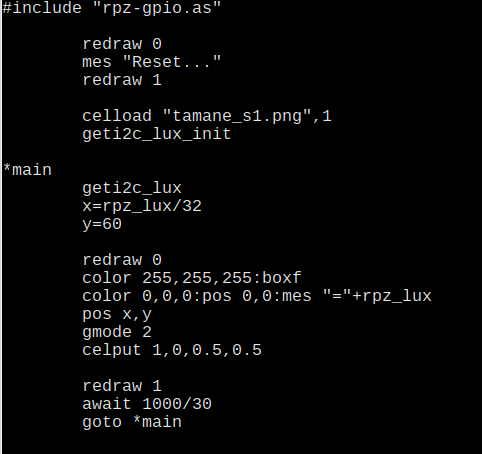
\includegraphics[keepaspectratio,width=11.615cm,height=10.94cm]{text04-img/text04-img040.png}
    \end{center}
    \label{fig:prog_menu}
\end{figure}

左上に表示されている数値が照度センサーの値です。

明るい時ほど大きい数字になるのがわかりますか?

自分の手でセンサーを覆ったり、光を当ててみたりしながら値が変わることを確認してみましょう。

確認ができたら、move.hspのプログラムを改造して、りんごの絵を照度センサーの値によって動かせるようにしてみましょう。


\begin{description}
    \item \textgt{\bf 例題4-13 答え}
\end{description}


「geti2c\_lux\_init」命令を最初に入れて1回だけ\ruby{初期化}{しょ|き|か}(準備)を行います。

その後、一定時間ごとに「geti2c\_lux」命令を実行することで、rpz\_luxという変数にセンサーの値が代入されます。

後は、rpz\_luxという変数の値をもとにプログラムで\ruby{処理}{しょ|り}を行います。

改造ができたらTAや周りの友達にも見せてあげましょう。

%2785